\chapter[Анализ состояния проблемы. Постановка задачи исследования]{%
  Анализ состояния проблемы. \hspace{2cm}
  Постановка задачи исследования
}

\section[История развития проблемы идентификации стохастических систем]{%
  \color{red} История развития проблемы идентификации \\
  стохастических систем
}

Начало идентификации систем, как предмета построения математических моделей на основе наблюдений,
связано с работами~\cite{gauss_1809, gauss_1810, gauss_1821} Гаусса,
в которых он разработал метод наименьших квадратов и использовал его для предсказания
траектории движения планет.
Впоследствии этот метод нашёл применение во множестве других приложений,
в том числе для построения математических моделей управляемых объектов,
используемых в автоматизации.
Существенный вклад в развитие метода наименьших квадратов внесли
Лаплас~\cite{laplace_1812}, Чебышев~\cite{chebyshev_1859}, Марков~\cite{markov_1898},
Эйткен~\cite{aitken_1935}, Колмогоров~\cite{kolmogorov_1946} и Рао~\cite{rao_1946}.
Системное изложение этого метода представлено, например, в работе Линника~\cite{linnik62}.

Большая часть ранних работ по идентификации систем была сделана специалистами в области статистики,
эконометрики (особенно их интересовали приложения идентификации, связанные с временными рядами) и
образовала область под названием статистическое оценивание.
{\color{red} Проблема заключалась в том, что область приложений этих методов была ограничена чаще всего
скалярными системами.}
В 1960 году Калман представил описание управляемой системы в
виде пространства состояний, что позволяло работать и с многомерными системами,
и заложил основы для оптимальной фильтрации и оптимального управления,
основывавшихся на данном типе описания.

Методы идентификации систем для задач управления были разработаны в 1965 году в работах
Хо и Калмана~\cite{ho_1965}, Острёма и Болина~\cite{astrom_1965}.
Работа Хо и Калмана посвящена поиску модели изучаемого объекта в пространстве состояний,
имеющей наименьший порядок вектора состояний, на основе информации об импульсной переходной характеристике.
Данная задача, но уже при наличии реализаций случайного процесса, где формируется марковская модель,
была решена в 70-х годах в работах Форре~\cite{faurre_1973} и Акайка~\cite{akaike_1974}.
Эти работы заложили создание метода подпространства в начале 90-х.

Работа Острёма и Болина представила для сообщества специалистов по идентификации метод
максимального правдоподобия, который был разработан специалистами по временным рядам для
оценивания параметров моделей в виде разностных уравнений~\cite{koopmans_1950}.
Эти модели, которые известны в статистической литературе как ARMA (авторегрессионное скользящее среднее) и
ARMAX (авторегрессионное скользящее среднее со входом), позднее,
образовали основу для создания метода ошибки предсказания.
В 1970-х годах этот метод стал доминировать в теории и, что более важно, в приложениях идентификации.
Большая часть исследовательской активности сфокусировалась на проблемах идентификации многомерных и
замкнутых систем.
Ключевой задачей для этих двух классов систем являлось найти условия для эксперимента и
способы параметризации проблемы, при которых найденная модель приблизится к единственно точному
описанию реальной системы.

К 1976 году была сделана первая попытка рассмотреть идентификацию систем как теорию аппроксимации,
в которой стоит задача наилучшей возможной аппроксимации реальной системы внутри данного класса
моделей~\cite{ljung_1976, anderson_1978, ljung_1979}.
Таким образом, преобладающая точка зрения среди специалистов по идентификации сменилась с
поиска описания для истинной системы на поиск описания наилучшей возможной аппроксимации.

Идея, что качество модели может быть изменено с помощью выбора переменных синтеза,
привела к всплеску активности в 90-х годах XX века, который продолжается до сих пор.
Главное применение новой парадигмы --- это идентификация для MBC (управление на основе модели).
Идентификация для задач управления расцвела с небывалой силой со времени своего появления и
применение к управлению методов идентификации вдохнуло вторую жизнь в такие уже
известные области исследования, как планирование эксперимента, идентификация в замкнутом контуре,
частотная идентификация, робастное управление при наличии неопределенности.

{\color{red}
  Как обстоят дела в СССР и СНГ?
  Нужно написать что-то о нашей работе.
}

\section[Идентификация стохастических систем как математическая проблема]{%
  Идентификация стохастических систем как \\
  математическая проблема}

\subsection{Постановка задачи идентификации}

Задача идентификации в общем виде формулируется следующим образом:
на основании априорной информации, а также по результатам наблюдений над
входными и выходными переменными системы должна быть построена оптимальная в
некотором смысле модель, т.~е. формализованное представление этой системы~\cite{eikhoff_1975}.

В зависимости от характера располагаемой априорной информации различают
задачи идентификации систем в узком и широком смысле.
Задача идентификации в узком смысле состоит в оценивании параметров и
состояния системы по результатам наблюдений над входными и выходными переменными,
полученными в условиях функционирования объекта.
При этом известна структура системы и задан класс, к которому эта модель относится.

В случае, когда априорная информация об объекте при идентификации в широком смысле отсутствует
или очень бедная, принято говорить о задаче идентификации в широком смысле.
При её решении приходится решать большое число дополнительных задач:
выбор структуры системы и задание класса моделей,
оценивание степени стационарности, линейности объекта и действующих переменных,
оценивание степени и формы влияния входных переменных на выходные,
выбор информативных переменных и др.

Стохастическая система --- система, связь входа и выхода которой имеет недетерминированный
(стохастический) характер. Это может быть обусловлено как недетерминированностью самой системы,
так и ошибками измерения её переменных.
Основными источниками таких ошибок являются:
ошибки, вызванные помехами;
ошибки усечения;
ошибки из-за неправильного определения состояния;
ошибки, связанные с упрощением при реализации;
ошибки выборочной аппроксимации~\cite{eikhoff_1975}.

{\color{red} Предметом данной работы является идентификация стохастических систем в узком смысле.
Данный выбор обусловлен следующими причинами.
Поскольку вход и выход реальных систем всегда измеряется с ограниченной точностью,
при идентификации удобно считать сами эти системы стохастическими.
Кроме этого, решение задачи идентификации в узком смысле необходимо для
решения задачи идентификации в широком смысле.
Наконец, задача идентификации в узком смысле является строго формализуемой.}

Математическая модель задачи идентификации имеет следующий вид:
\begin{equation}
  \label{eq:model_general}
  \begin{aligned}
    H &= \Psi (\Theta, \Xi), \\
    X &= \Xi + E_x, \\
    Y &= H + E_y,
  \end{aligned}
\end{equation}
где \( \Xi, H \) --- векторы фактических значений входной и выходной переменной, \par
\( \Theta \) --- вектор фактических значений параметров объекта, \par
\( \Psi \) --- векторная функция регрессии, \par
\( X, Y \) ---  вектор измеренных значений входной и выходной переменной, \par
\( E_x, E_y \) --- векторы независимых ошибки измерений значений входной и выходной переменной,
распределенные по нормальному закону:
{\color{red} \( E_x = N(0, \sigma_{E_x}), E_y = N(0, \sigma_{E_y}) \)}.

В этой задаче требуется,
считая вид функции \( \Psi \) известными и располагая измеренными значениями входа и выхода \( X, Y \),
найти оценку $ \hat{\Theta} $ вектора параметров системы $ \Theta $.

Следует отметить, что в ряде частных случаев данная модель имеет более простой вид.
Так, например, в скалярном случае, когда система имеет всего один вход и выход,
модель~\ref{eq:model_general} сводится к
\begin{equation}
  \label{eq:model_scalar}
  \begin{aligned}
    h &= \psi (\theta_1, \ldots, \theta_n, \xi), \\
    x &= \xi + e_x, \\
    y &= h + e_y,
  \end{aligned}
\end{equation}
где \( \xi, H \) --- фактические значения входной и выходной переменной, \par
\( \theta \) --- фактические значения параметров объекта, \par
\( \psi \) --- скалярная функция регрессии, \par
\( x, y \) --- измеренные значения входной и выходной переменной, \par
\( e_x, e_y \) --- независимые ошибки измерений значений входной и выходной переменной,
распределенные по нормальному закону: \( e_x = N(0, \sigma_{e_x}), e_y = N(0, \sigma_{e_y}) \).

Если же скалярная система~\ref{eq:model_scalar} является к тому же линейной,
то её модель можно записать в еще более простом виде:
\begin{equation}
  \label{eq:model_scalar_linear}
  \begin{aligned}
    h &= \psi (\alpha, \beta, \xi), \\
    x &= \xi + e_x, \\
    y &= h + e_y,
  \end{aligned}
\end{equation}
где \( \alpha, \beta \) --- фактические значения параметров объекта.

\subsection{Классификация стохастических систем}

{\color{red} Статистические данные могут порождаться системами нескольких видов.}
{\color{red} TODO: проверить обозначения}.

Полустохастическим объектом будем называть объект с детерминированным входом и случайным выходом.
Это либо регрессионный объект (объект с внутренним шумом на выходе),
либо детерминированный объект с ошибками в измерениях выходных переменных (рисунок~\ref{fig:type_half}).

\begin{figure}[h!]
  \centering
  \fcolorbox{gray}{white}{
    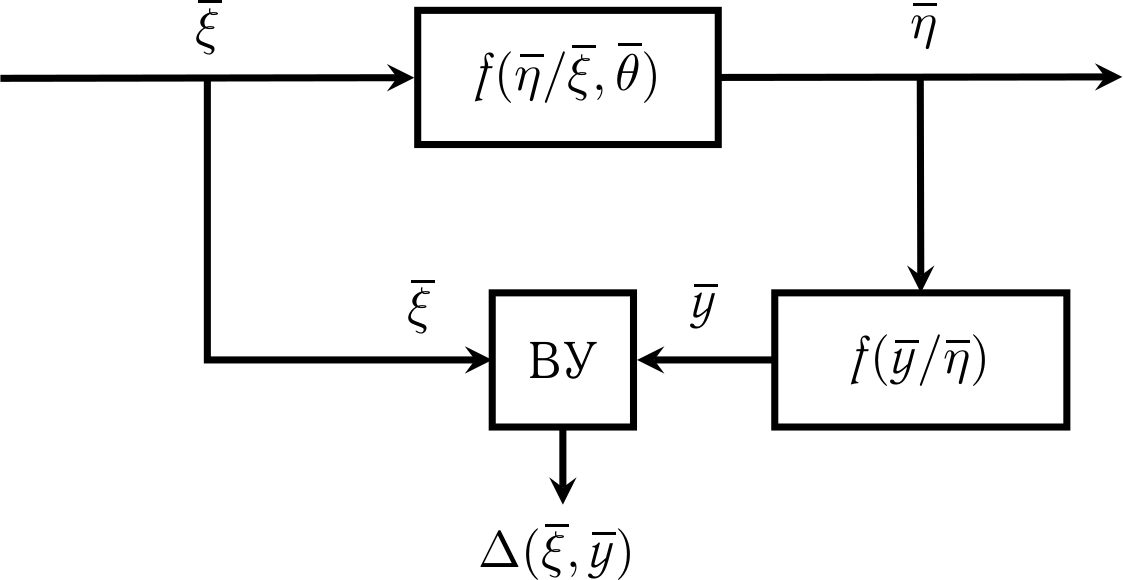
\includegraphics[width=92mm]{fig/half_new.png}
  }
  \caption{Схема полустохастического объекта}
  \label{fig:type_half}
\end{figure}

Объект описывается условной плотностью вероятности \( f(\eta / \xi, \theta) \),
\( \eta \) --- выходная переменная,
\( \xi \) --- входная переменная,
\( \theta \) --- параметр объекта,
\( y \) --- наблюдение выходной переменной,
\( f(y / \eta) \) --- условная плотность вероятности, описывающая измерительную систему,
ВУ --- вычислительное устройство,
\( \Delta(\xi, y) \) --- результат аппроксимации.
Входная и выходная переменная, а также параметр могут быть многомерными.

Стохастическим объектом первого типа будем называть объект со случайным входом и выходом
(рисунок~\ref{fig:type_first}).
Объект описывается совместной плотностью вероятности \( f(\xi, \eta) \).
Возможно наличие ошибок в измерениях входных и выходных переменных.

\begin{figure}[h!]
  \centering
  \fcolorbox{gray}{white}{
    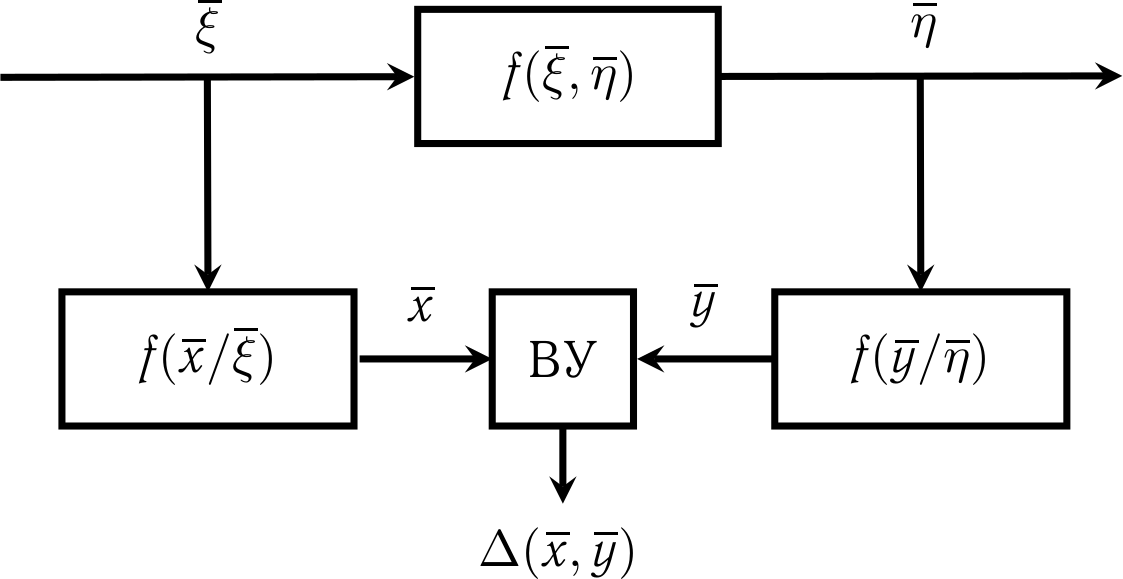
\includegraphics[width=92mm]{fig/first_new.png}
  }
  \caption{Схема стохастического объекта \\ первого типа}
  \label{fig:type_first}
\end{figure}

Стохастическим объектом второго типа назовем детерминированный объект с ошибками
в измерениях входных и выходных переменных (рисунок~\ref{fig:type_second}).
Объект описывается детерминированной зависимостью \( \eta = \phi(\xi, \theta), \)
\( \theta \) --- вектор параметров объекта.

\begin{figure}[h!]
  \centering
  \fcolorbox{gray}{white}{
    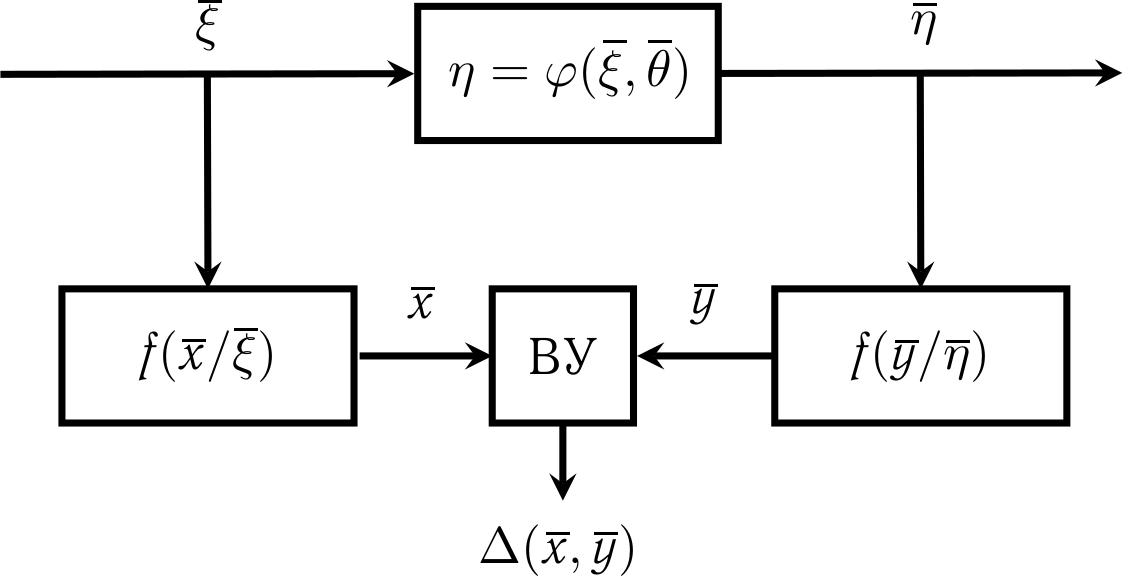
\includegraphics[width=92mm]{fig/second_new.png}
  }
  \caption{Схема стохастического объекта \\ второго типа}
  \label{fig:type_second}
\end{figure}

\newpage
\subsection{Критерии идентификации стохастических систем}

Критерием выбора оптимума должен быть функционал от выходных
сигналов или от математического ожидания ошибок оценок параметров.

Как оценить точность идентификации -- по отклонениям параметров
модели или её отклика? Если основная цель состоит в
проектировании системы управления, то представляется логичным
оценивать точность идентификации по результатам функционирования
созданной на основе идентификации объекта системы управления~\cite{eikhoff_1975}.

В настоящее время наиболее широкое распространение получил критерий
минимума суммы квадратов вертикальных расстояний от наблюдений выходной переменной
до аппроксимирующей прямой или плоскости (классический критерий наименьших квадратов).
Этот критерий формально применим ко всем вида рассмотренных выше объектов.

Известен также другой критерий, состоящий в минимизации суммы квадратов
перпендикулярных расстояний от наблюдений входных и выходных переменных до
аппроксимирующей прямой или плоскости~\cite{pearson_1901, mukha_2016}.

Области предпочтительного использования названных выше критериев
достаточно четко не определены.

Относительно задачи линейной аппроксимации полустохастического объекта
можно сказать, что она полностью решена в рамках классического линейного
регрессионного анализа как задача оценивания параметров линейной математической модели
объекта с критерием минимизации суммы квадратов вертикальных расстояний.
Оптимальное решение здесь --- классическая линейная регрессия,
обеспечивающая как оптимальное оценивание параметров математической модели объекта
(при заданных значениях входных переменных),
так и оптимальное прогнозирование наблюдений выходных переменных
по наблюдениям входныхх переменных.

\section{Постановка задачи исследования}

% Теория идентификации систем, рассматривающая данную задачу,
% получила свое наибольшее развитие во второй половине XX века.
% Её выводы находят свое применение в различных отраслях науки и техники:
% энергетике, машиностроении, авиации, химической промышленности,
% физике, экономике, биологии и медицине при решении таких прикладных задач, как
% диагностика, управление, автоматический контроль,
% автоматизация принятия решений, распознавание образов.
% Данная теория опирается на следующие дисциплины:
% метрологию, теории управления, систем, сигналов, информации,
% стохастическую аппроксимацию и математическую статистику~\cite{eikhoff_1975}.


% Построение модели сводится к следующим этапам:
% \begin{itemize}
% \item выбор структуры модели из физических соображений;
% \item подгонка параметров к имеющимся данным (оценивание);
% \item проверка и подтверждение модели (диагностическая проверка);
% \item испольование модели по назначению.
% \end{itemize}

% Структура модели выбирается на основе априорной информации о системе и
% преследуемых целях.

% В большинстве реальных ситуаций налюдения над системой искажены
% случайными воздествиями (возмущениями, ошибками).

% Под оцениванием параметров понимается экспериментальное определение
% значений параметров, характеризующих динамику поведения объекта,
% в предположении, что структура модели объекта известна.

% Как оценить точность идентификации -- по отклонениям параметров
% модели или её отклика? Если основная цель состоит в
% проектировании системы управления, то представляется логичным
% оценивать точность идентификации по результатам функционирования
% созданной на основе идентификации объекта системы управления.

% теория систем -- линейные и нелинейные модели
% теоретическая дисциплина -- стохастическая аппроксимация ?
% цели применения.

% Выбор между линейными и нелинейными моделями.
% Скорость изменения параметров?
% Выбор типа модели тесно связан с решаемой задачей.

% Два вида реализаций:
% - использующая явные математические выражения;
% - реализации по настраиваемой модели.

% Методы идентификации:
% - вне контура регулирования;
% - внутри замкнутого контура регулирования.

% Дополнительная априорная информация приводит к улучшению оценик,
% однако затраты на реализацию могут оказаться чрезмерными.

% Метод наименьших квадратов может быть получен из метода максимума правдоподобия.

% Есть ли связь между НМНК и марковскими оценками?

% В обзоре литературы, охватывающем не менее 30 источников за последние 10–15 лет (включая зарубежные публикации и электронные ресурсы), необходимо показать основные этапы в развитии знания по проблеме диссертации, критически осветив известные работы, необходимо назвать неразрешенные вопросы и таким образом определить свое место в решении проблемы. Желательно закончить этот раздел кратким резюме о той конкретной задаче, которую автор стремиться поставить и решить в диссертации.



% Это вызвано тем, что она является неотъемлемой частью задачи идентификации
% в широком смысле, а также поддаётся полной формализации.

% Для идентификации стохастических систем можно использовать математические методы
% аппроксимации статистических данных.



% https://ru.wikipedia.org/wiki/%D0%98%D0%B4%D0%B5%D0%BD%D1%82%D0%B8%D1%84%D0%B8%D0%BA%D0%B0%D1%86%D0%B8%D1%8F_%D1%81%D0%B8%D1%81%D1%82%D0%B5%D0%BC#CITEREFРастригин1977